\clearpage
\section*{Write Back}
The Write Back stage will allow for the writing to the register file. It takes \verb+iCode+, \verb+rA+, and \verb+rB+ as inputs and outputs \verb+dstE+ and \verb+dstM+.

\subsection*{Contributors}
Huy Lai\\
Arjun Kurkal
\subsection*{Screenshots}
\begin{figure}[!ht]
    \centering
    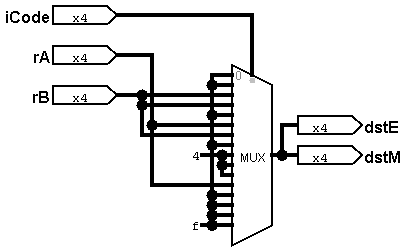
\includegraphics[width=\textwidth]{Images/WriteBack.png}
    \caption{Write Back}
\end{figure}

\clearpage
\section*{PC Update}
The PC Update stage will tell the PC where to go next. It takes \verb+iCode+, \verb+valP+, \verb+valM+, \verb+valC+ along with \verb+cnd+ from the Execute stage as inputs. \verb+cnd+ is used on \verb+jXX+, when high this indicates that a jump is being made.
\subsection*{Contributors}
Huy Lai\\
Arjun Kurkal\\
Kyle Crusius

\subsection*{Screenshots}
\begin{figure}[!ht]
    \centering
    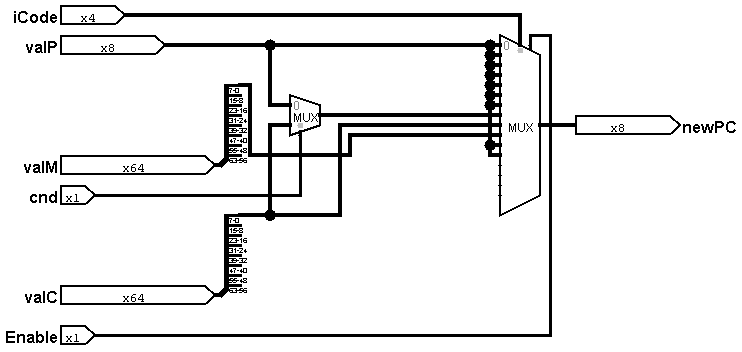
\includegraphics[width=\textwidth]{Images/PCUpdate.png}
    \caption{PC Update}
\end{figure}